\documentclass[12pt,modern]{aastex61}
\usepackage{graphics,graphicx}
\usepackage{hyperref}
\usepackage{amssymb}
\usepackage{amsmath}
\usepackage{comment}


\shortauthors{Bouma, Winn, Masuda}
\shorttitle{Binarity and Occurrence Rates}

\begin{document}
    
\title{ The effects of binarity on planet occurrence rates measured by transit 
surveys}

\author{
L. G. Bouma, J. N. Winn, K. Masuda
}

\begin{abstract}

This work aims to clarify the biases that stellar binarity introduces
to occurrence rates inferred from transit surveys.
In general, stellar multiplicity leads to diluted planetary 
radii, overestimated detection efficiencies, and an undercounted number of 
selected stars (but possibly an overcounted number of searched stars).
These effects skew occurrence rate measurements in different directions, and 
we develop simple models that allow us to understand the crucial effects.
For a model in which all stellar systems are either single or twin binaries, 
and all planets are identical, we find that ignoring binarity leads to an 
underestimate of the occurrence at the true radius by a multiplicative factor 
of $0.8$ (assuming a 10\% twin binary fraction).
Using more realistic models for the stellar population and planetary 
radii, we find that ignoring binarity leads to a $10$\,-\,$30\%$ 
underestimate of the number of planets per star, depending on the true radius 
distribution.
For the occurrence of Earth-sized planets, in our most realistic model the 
underestimate is by $\approx 15\%$~--~at present far smaller than 
systematic uncertainties on real $\eta_\oplus$ measurements.
For hot Jupiters, we find that the inferred occurrence rate is 
$\approx 1.3\times$ smaller than the true rate around single stars.
We suggest that this latter effect contributes to the discrepant hot Jupiter 
rates measured by {\it Kepler}\ and the California group's respective surveys.
\end{abstract}

\section{Introduction}

An astronomer who does not believe in stellar multiplicity wants to measure the
mean number of planets of a certain type per star of a certain type.
They perform a signal-to-noise limited transit survey and detect $N_{\rm det}$ 
transit signals that appear to be from planets of the desired type.  They 
calculate the apparent number of searchable stars, $N_\star$.  ``Searchable 
stars'' are the stars for which 
planets are observed with 100\% detection efficiency. 
Correcting for the geometric 
transit probability $f_{\rm g}$, they compute an apparent occurrence rate 
$\Lambda_{\rm a}$:

\begin{equation}
\Lambda_{\rm a} = \frac{N_{\rm det}}{N_\star} \times \frac{1}{f_g}.
\end{equation}

There are many potential pitfalls.  Some genuine transit signals can be missed
by the detection pipeline.  Some apparent transit signals are spurious, from
noise fluctuations, failures of `detrending', or instrumental effects.  Stars
and planets can be misclassified due to statistical and systematic errors in
the measurements of their properties.  Poor angular resolution causes false
positives due to blends with background eclipsing binaries. {\it Et cetera}.

Here we focus on problems that arise from the fact that many stars exist in 
multiple star systems.
For simplicity, we only consider binaries, and we assume that they are all 
spatially unresolved.

An immediate complication is that, due to dynamical stability or some 
aspect of planet formation, the occurrence rate of planets may differ 
between binary and single-star systems.
If ``occurrence rate'' is defined purely as the mean number of planets within 
set radius and period bounds per star in a given mass interval, it must 
implicitly marginalize over stellar multiplicity.
This means marginalizing over ``occurrence rates in single star systems'', 
``occurrence rates about primaries'', and
``occurrence rates about secondaries'' (see {\it e.g.,} Wang et al., 
2015).

Outside of astrophysical differences, there are observational biases.
A given apparently-searchable star may truly be a single star of the desired 
type. If it is binary, it may contain two, one, or no searchable stars of the 
desired type, which affects $N_\star$.
There may be systematic errors in stellar parameter estimates of such 
systems, which in this work we neglect.
One might also imagine an apparently-searchable star which in no stellar 
component is of the desired type. We will not consider errors of this type.  
We will assume that all the apparently-searchable stars are either single 
stars of the desired type, or binaries in which either the primary or else 
both components are of the desired type.

When counting the detected signals from planets of the desired 
type, $N_{\rm det}$, ignoring binarity leads to errors in planet radius 
classification, and the assumed survey completeness.
Detected planets in binary systems will have underestimated radii because of 
the diluting flux from the companions, and possibly because they are assumed 
to orbit the wrong star ({\it e.g.}, Furlan et al. 2017).
The number of selected stars should change dependent on the planet radius 
and period for which the rate measurement is desired, and on the survey's 
achieved photometric precision.
This means our naive astronomer assumes the fraction of their selected stars 
which are searchable is 1 (this is their ``assumed completeness'').
Binarity confuses this, because the ability to search for planets 
in binary systems depends on which stellar component hosts the planet, and on 
how much dilution affects the measurement.

\paragraph{How Has Binarity Been Considered in Occurrence Rate Measurements?}
Many authors have reported planet occurrence rates from transit 
survey data\footnote{
    An online list of occurrence rate papers is maintained at 
    \url{https://exoplanetarchive.ipac.caltech.edu/docs/occurrence_rate_papers.html}
}.
With regard to binarity, the typical approach has been to ignore the 
issue\footnote{Deacon et al., 2015 are an exception to the rule.}.
For instance, in a laudable study by Burke et al. (2015), they
\begin{quote}
``treat the pipeline completeness as having no uncertainty 
due to the incomplete understanding of the stellar parameters, eccentricity, 
and stellar binarity.''
\end{quote}
Though they do ``explore sensitivity in the derived planet occurrence rates 
to alternative assumptions for the stellar parameters and non-zero 
eccentricities'', they do not for binarity.

Of course, on a system-by-system level stellar multiplicity affects the 
interpretation of planet candidates. High resolution imaging 
campaigns have consequently been undertaken to measure the multiplicity of 
almost all {\it Kepler}\ Objects of Interest 
(Howell et al. 2011; Adams et al. 2012, 2013; Horch et al. 2012, 2014; 
Lillo-Box et al. 2012, 2014; Dressing et al. 2014; Law et al. 2014; Cartier et 
al. 2015; Everett et al. 2015; Gilliland et al. 2015; Wang et al. 2015a, 
2015b; Baranec et al. 2016).
The results of these programs have been collected by Furlan et al. 
(2017), and they represent an important advance in understanding the KOI 
sample's multiplicity statistics.
In particular, they can be immediately applied to rectify binarity's influence 
on the mass-radius diagram (Furlan \& Howell 2017).

For {\it Kepler}-derived occurrence rates, the high resolution imaging 
campaigns have not yet come full circle to observe a comparison sample of 
non-KOI host stars.
The most recent rate studies have thus used Furlan et al. (2017)'s 
catalog to test the effects of removing KOI hosts with known companions, which 
is an important step towards reducing contamination in the ``numerator'' of 
the occurrence rate (Fulton et al. 2017).
However, without an understanding of the multiplicity statistics of the 
non-KOI hosting stars that are assumed to be searchable, the 
true completeness, the true number of searchable stars, and thus the true 
occurrence rates will remain uncertain.


\paragraph{The Hot Jupiter Rate Discrepancy}
There is at least one context in which measurement of absolute 
occurrence rates may already be showing the signatures of binarity.
Hot Jupiter occurrence rates measured by transit surveys ($\approx 0.5\%$) are 
marginally lower than those found by radial velocity surveys ($\approx 1\%$; 
see Table~\ref{tab:hj_rates}).
Though the discrepancy is of weak statistical significance ($<3\sigma$),
one plausible explanation for the difference is that the populations have 
distinct metallicities.
As originally argued by Gould et al. (2006), the RV sample is biased towards 
metal-rich stars, which have been measured by RV surveys to preferentially 
host more giant planets (Santos et al 2004, Fischer and Valenti 2005).
The {\it Kepler}\ sample specifically has been measured to be more metal poor 
than the local neighborhood, with a mean metallicity of $[{\rm M/H}]_{\rm 
mean}\approx -0.05$ (Dong et al., 2014; Guo et al., 2017).
Studying the problem in detail, Guo et al. recently argued that the 
metallicity difference could account for a $\approx 0.1\%$ difference in the 
measured rates between the CKS and {\it Kepler}\ samples~--~not a $\approx 
0.5\%$ difference.
Guo et al. concluded that ``other factors, such as binary contamination and 
imperfect stellar properties'' must also be at play.

Aside from surveying stars of varying metallicities, radial velocity and 
transit surveys differ in how they treat binarity.
Radial velocity surveys typically reject both visual and spectroscopic binaries
({\it e.g.}, Wright et al. 2012).
Transit surveys typically observe binaries, but the question of whether they 
were searchable to begin with is usually left for later interpretation.
In spectroscopic follow-up of candidate transiting planets, the prevalence of 
astrophysical false-positives may also lead to a bias against confirmation of 
transiting planets in binary systems.

Ignoring these complications, in this work we focus on whether
binarity might intrinsically bias transit survey occurrence rates, simply 
through its effects on the number of searchable stars and the apparent radii 
of detected planets.

To progressively gain intuition, we study the following idealized transit 
surveys:
\begin{itemize}
    \item Model \#1: fixed stars, fixed planets, twin binaries;
    \item Model \#2: fixed planets and primaries, varying secondaries;
    \item Model \#3: fixed primaries, varying planets and secondaries.
\end{itemize}
In Sec.~\ref{sec:numerical_methods}, we introduce our numerical approach 
to the problem, and in Sec.~\ref{sec:analytic_preliminaries} we clarify our 
terminology.
We present the analytic and numerical results in 
Secs.~\ref{sec:model_1}-\ref{sec:model_3}, where each subsection corresponds 
to each model above.
We interpret these calculations throughout, and in 
Sec.~\ref{sec:discussion} discuss their relevance to various questions in 
the interpretation of transit survey occurrence rates. 

\section{Method}

\subsection{Numerical Approach}
\label{sec:numerical_methods}

Assuming a signal-to-noise limited survey, we would like to find the true
occurrence rate density, and also that inferred by an observer ignoring 
binarity.
Though analytic or semi-analytic solutions exist for each model, beyond Model 
\#2 the equations become burdensome. To maintain simplicity, we develop a 
Monte Carlo approach, which works as follows.

First, the user specifies the model class (\#1, 2, or 3) and various free 
parameters describing the stellar and planetary population.
Most importantly, these parameters include the binary fraction, and the true 
planet occurrence rates around single stars, primaries, and secondaries (the 
$\Lambda_i$'s, to be defined in Sec.~\ref{sec:analytic_preliminaries}).
                                                               
We then generate the population of selected stars.
Each selected star has a type (single, primary, secondary), 
a binary mass ratio (if it is not single), and the property of whether it 
is ``searchable''.               
The absolute number of stars is arbitrary.
The relative number of binaries to singles is calculated according to analytic
formulae. The binary mass ratios are sampled from the
appropriate magnitude-limited distributions.

Whether a star is ``searchable'' depends entirely on its ``completeness''
fraction. By ``completeness'', we mean the ratio of the actual number of 
searchable stars to the assumed number of searchable stars (for a given planet 
size, period, etc.).
Assuming homogeneously distributed stars, this is equivalent to the
ratio of the searchable to selected volumes.
For single stars, we assume these volumes are identical~--~exactly the case 
discussed by Pepper et al. (2003).
For binaries, this volume ratio is a function of only the binary mass ratio.

To assign planets, each selected star receives a planet at the initially 
specified rate, according to its type.
The radii of planets are assigned independently of any host system
property, as sampled from $p_r(r) \sim r^\delta$ for Model \#3 or a 
$\delta$--function 
for Models \#1 and \#2.
A planet is detected when a) it transits, and b) its host star is
searchable.

The probability of transiting single stars in our model is assumed to be known,
and so it is mostly corrected by the observer attempting to infer an
occurrence rate. The only bias is for secondaries, which can be smaller than 
primaries in Models \#2 and \#3.
This effect is included when computing the transit probability.

For detected planets, apparent radii are computed according to analytic
formulae that account for both dilution and the misclassification of stellar
radii. We assume that the observer think all transits are around single 
stars.

The rates are then computed in bins of true planet radius and apparent planet
radius.
In a given radius bin, the true rate is found by counting the number of planets
that exist around selected stars of all types (singles, primaries,
secondaries), and dividing by the total number of these stars.
The apparent rates are found by counting the number of detected planets that
were found in an apparent radius bin, dividing by the geometric transit
probability for single stars, and dividing by the apparent total number of
stars.
The simplest realization of this scheme is described analytically in 
Sec.~\ref{sec:model_1}, but we first clarify our terminology.

\subsection{Analytic Preliminaries}
\label{sec:analytic_preliminaries}

Define the occurrence rate density, $\Gamma$,
as the expected number of planets per star per natural logarithmic bin 
of planetary and stellar phase space:
\begin{equation}
\Gamma(\vec{x}) = \frac{d^n\Lambda}{\prod_{i=1}^{n} {\rm d} \ln x_i  }.
\label{eq:rate_density_defn}
\end{equation}
$\vec{x}$ is an $n$-dimensional list of the continuous physical properties 
that might affect the occurrence rate density. 
For example,
$\vec{x}=(r,P,R)$ where $r$ is the planet radius, $P$ is its orbital period, 
and $R$ is the host star radius.
The occurrence rate $\Lambda$ is found by integrating the rate density over a 
specified volume of phase space (e.g., Youdin 2011).


The previous definition implicitly marginalizes the rate density over stellar 
multiplicity.
For simplicity, this work only considers single and binary star systems.
Then for a selected population of stars and planets the rate density can be 
written\footnote{
    Eq.~\ref{eq:rate_density_marginalized} follows by writing the $i^{\rm 
        th}$ system type's rate density as some normalization multiplied by a 
    probability density:
    $\Gamma_i(\vec{x}) = \mathcal{Z}_i p_i(\vec{x})$.
    For Eq.~\ref{eq:rate_density_defn} to hold, we must have $\mathcal{Z}_i = 
    \Lambda_i$.
}
\begin{equation}
\Gamma(\vec{x})
= \sum_{i=0}^{2} w_i \Gamma_i(\vec{x})
= \sum_i w_i \Lambda_i p_i(\vec{x})
\label{eq:rate_density_marginalized}
\end{equation}
where $i=0$ corresponds to single star systems, $i=1$ primaries of binaries, 
and $i=2$ secondaries of binaries.
$\Lambda_i$ is the occurrence rate integrated over all possible phase space  
for the $i^{\rm th}$ system type, and $p_i(\vec{x})$ is the joint 
probability density function so that $\Gamma_i(\vec{x}) = \Lambda_i 
p_i(\vec{x})$.
The weights are given by 
\begin{equation}
w_i = N_i/N_{\rm tot},
\end{equation}
for $N_{\rm tot} = \sum_i N_i$ the total number of selected stars, and 
$N_0,N_1,N_2$ the number of selected single stars, primaries, and 
secondaries respectively.
Both $N_1$ and $N_2$ are equal to the number of selected points on 
the sky which are in fact binary systems.
The relationship between the rate $\Lambda$ over a desired volume of 
phase space $\Omega_{\rm desired}$ and $\Lambda_i$ is
\begin{equation}
\Lambda = \sum_i
\left(
w_i \Lambda_i \int_{\Omega_{\rm desired}} p_i(\vec{x}) \,{\rm d}\Omega
\right),
\label{eq:occ_rate}
\end{equation}
where $p_i(\vec{x})$ is assumed to be normalized to unity.

A transit survey will have a rate density of detected planets $\hat{\Gamma}$, 
which for each system type will be the product of the rate density and the 
detection efficiency $Q_i(\vec{x})$:
\begin{equation}
\hat{\Gamma}(\vec{x}) = \sum_i Q_i(\vec{x}) \Gamma_i(\vec{x}) 
\equiv \sum_i \hat{\Gamma}_i(\vec{x}),
\label{eq:detected_rate_density}
\end{equation}
where again the index $i$ is over each type of system (singles, primaries, 
and secondaries).
The detection efficiency includes the geometric transit probability, as well 
as any incompleteness effects.
Foreman-Mackey et al. (2014) discuss how this 
is calculated in practice.



\section{Analytic and Numerical Results}

%\subsection{Model \#1: fixed stars, fixed planets, twin binaries}
\label{sec:model_1}

Since the effects of binarity are most pronounced when the two components are 
similar, we begin by considering a universe in which all planets are 
identical, and all stars are either single or twin stars with otherwise 
identical physical properties.
The occurrence rate density at a planet radius $r$, stellar radius $R$, and 
semimajor axis $a$ for this model is
\begin{equation}
\Gamma(r,R,a) = \sum_i w_i \Lambda_i \delta^3(r_p,R_\star,a_p),
\label{eq:model1_occ_rate_density}
\end{equation}
for $r_p$ and $R_\star$ some fixed planet and stellar radii, $a_p$ a fixed 
semi-major axis, and $\delta$ the Dirac delta function, whose compact
form will be used for brevity.
The occurrence rate over any interval that includes $r_p$, $R_\star$, and 
$a_p$ is
\begin{equation}
\Lambda = \sum_i w_i \Lambda_i = \frac{ \sum_i N_i \Lambda_i }{N_{\rm tot}}.
\end{equation}
The rate is zero over intervals that do not.

To express the rate density of detected planets, $\hat{\Gamma} = \sum 
Q_i\Gamma_i$, we need the detection efficiencies for each system type, which 
are products of the geometric and selection probabilities:
\begin{align}
Q_i(\vec{x}) &= Q_{g,i}(\vec{x}) Q_{c,i}(\vec{x}),\quad {\rm where}\ 
\vec{x}=(r,R,a).
\label{eq:general_detection_efficiency}
\end{align}
Similar to Pepper et al. (2003), but in a new context, we take $Q_c$ as the 
ratio of the number of stars that were searchable to the number of stars that 
were selected.
Assuming a homogeneous distribution of stars, this gives
\begin{equation}
Q_{c,i}(\vec{x}) = \left(
\frac{d_{{\rm det},i}(\vec{x})}{d_{\rm sel}(\vec{x})}
\right)^3,
\end{equation}
for $d_{\rm sel}$ the maximum distance to which surveyed stars are selected, 
and $d_{{\rm det},i}$ the maximum distance to which planets can actually be 
detected about the $i^{\rm th}$ system type.
Note that $d_{\rm sel} \geq d_{{\rm det},i}$.
In a signal-to-noise limited transit survey in which the observer does not 
know which stars are binaries, 
\begin{equation}
d_{\rm sel} \propto (r/R)^2 (L_{\rm sys} T_{\rm dur} A N_{\rm tra})^{1/2},
\end{equation}
for $L_{\rm sys}=L_1(1+\ell)$ the system luminosity, $T_{\rm dur}$ the 
transit duration, $A$ the detector area, and $N_{\rm tra}$ 
the number of observed transits.
However,
\begin{equation}
d_{{\rm det},i} \propto \mathcal{D}_i(r/R)^2 (L_{\rm sys} T_{\rm dur} A N_{\rm 
tra})^{1/2},
\label{eq:d_det_i}
\end{equation}
for the dilution $\mathcal{D}_i$ given by
\begin{align}
\mathcal{D}_i
&=
\left.
\begin{cases}
1 & \text{for } i=0,\ {\rm single} \\
L_1 / L_{\rm sys} = (1+\ell)^{-1}, & \text{for } i=1,\ {\rm primary} \\
\ell L_1 / L_{\rm sys} = (1 + \ell^{-1})^{-1}, & 
    \text{for } i=2,\ {\rm secondary},
\end{cases}
\right.
\label{eq:dilution}
\end{align}
where the light ratio $\ell$ of a given binary is defined as the ratio of 
the luminosity of the secondary to the primary.

The maximum detectable distance to single stars is assumed to be known, and so 
$d_{{\rm sel},0} = d_{{\rm det},0}$.
This means our naive astronomer assumes the fraction of their selected stars 
which are searchable is 1 (this is their ``assumed completeness'').
For binary systems there is a necessary incompleteness, and combining 
Eqs.~\ref{eq:general_detection_efficiency} through~\ref{eq:dilution} yields
\begin{align}
Q_0 &= Q_{g,0}Q_{c,0} = Q_{g,0} \label{eq:detection_efficiency_0}\\
Q_1 &= Q_{g,1}Q_{c,1} = Q_{g,0} (1+q^\alpha)^{-3} \\
Q_2 &= Q_{g,2}Q_{c,2} = Q_{g,0} q^{2/3} (1+q^{-\alpha})^{-3} q^{-5}, 
\label{eq:detection_efficiency_2}
\end{align}
for $Q_{g,0}=R/a$, the transit probability in single star systems.
In Eq.~\ref{eq:detection_efficiency_2}, we have assumed a stellar 
mass-luminosity-radius relation: $R\propto M \propto L^{1/\alpha}$.
The geometric transit probability is $Q_{g,2} = Q_{g,0}q^{2/3}$, and the 
completeness is the latter term of Eq.~\ref{eq:detection_efficiency_2}.
For $q=1$, the $q^{2/3}$ and $q^{-5}$ evaluate to unity, but they will later 
become relevant.

Summarizing, we have written the rate density for each system type
(Eq.~\ref{eq:model1_occ_rate_density}) and the detection efficiency for each 
system type 
(Eq.~\ref{eq:detection_efficiency_0}-\ref{eq:detection_efficiency_2}),
and so have fully specified the rate density of detected planets, 
in addition to the true rate density.


\paragraph{What does an observer ignoring binarity infer?} 
An observer who ignores binarity assumes a detection efficiency 
$\tilde{Q}=Q_0$,
measures a detected planet rate density $\tilde{\Gamma}$, 
and infers an apparent rate density $\Gamma_a$.
Analogous to Eq.~\ref{eq:detected_rate_density},
\begin{equation}
\tilde{\Gamma} = \Gamma_a \tilde{Q}.
\end{equation}
Accounting for dilution, and assuming $q=1$, the apparent rate density is
\begin{equation}
\Gamma_a = 
w_a \Lambda_0 \delta^3(r_p, R_\star, a_p) +
w_b (\Lambda_1 Q_{c,1} + \Lambda_2 Q_{c,2}) 
				\delta^3(r_p/\sqrt{2}, R_\star, a_p),
\end{equation}
for $w_a = N_0/(N_0+N_1)$, and $w_b = N_1/(N_0+N_1)$.
This observer miscounts the number of total searched stars, does not correct 
for incompleteness, and misclassifies the planetary radii because of dilution.

\paragraph{Correction to inferred rate density and inferred rate}

Define a rate density correction factor, $X_\Gamma$, as the ratio of the 
apparent to true rate densities:
\begin{equation}
X_\Gamma \equiv \frac{\Gamma_a}{\Gamma}.
\end{equation}
This factor can be a function of whatever parameters $\Gamma_a$ and $\Gamma$ 
depend on; in this study, the planet radius is most relevant.
For the twin-binaries model,
\begin{equation}
X_\Gamma(r)
=
\frac{w_a \Lambda_0\delta^3(r_p) + 
	w_b(\Lambda_1 Q_{c,1} + \Lambda_2 Q_{c,2}) \delta^3(r_p/\sqrt{2})  }
	{(w_0\Lambda_0 + w_1\Lambda_1 + w_2\Lambda_2)\delta^3(r_p)}
	\label{eq:model1_correction}
	\end{equation}
where $\delta^3(r_p)$ is shorthand for $\delta^3(r-r_p,R-R_\star,a-a_p)$.

If we take the rates $\Lambda_i$ to be equal, applying the definitions of 
the weights gives a rate density correction factor at $r=r_p$ of
$X_\Gamma(r_p) = (1+\mu)^{-1}$, where 
\begin{align}
\mu \equiv \frac{N_1}{N_0} &=
\frac{n_b}{n_s} \left(\frac{d_{\rm sel,b}}{d_{\rm sel,s}}\right)^3 = 
\frac{{\rm BF}}{1-{\rm BF}} (1+\ell)^{3/2},
\label{eq:mu_definition}
\end{align}
for $n_b$ and $n_s$ the number density of binaries and singles in a 
volume limited sample.
Using Raghavan et al. (2010)'s $0.7-1.3M_\odot$ multiplicity fraction as our 
binary fraction\footnote{
The binary fraction is the fraction of systems in a volume-limited sample that 
are binary. It is equivalent to the multiplicity fraction if there are no 
triple, quadruple, or higher order multiples. In that case, ${\rm BF} = n_b / 
(n_s+n_b)$.
}, we set ${\rm BF}=0.44$.
The resulting correction to the rate density is $X_\Gamma(r_p) \approx 0.31$. 
The correction at $r_p/\sqrt{2}$ is infinite.
The numerical realization of this model agrees with these analytic values, and 
its output is shown in Fig~\ref{fig:errcases_model_1}.
%beta = 2.2223355980148636
If instead we assume that $\Lambda_0 = \Lambda_1$, but that $\Lambda_2=0$, we 
find 
$X_\Gamma(r_p) = (1+2\mu)/(1+\mu)^2$.
Taking the same binary fraction, this evaluates to $X_\Gamma(r_p)\approx 0.53$.
Since the correction to the rate is equal to that of rate density, at 
$r=r_p$, the occurrence rate is underestimated by a factor of roughly 2 to 3.

%Note that a correction to the inferred rate, $X_\Lambda$, can be 
%defined analogously:
%\begin{equation}
%X_\Lambda \equiv \frac{\Lambda_a}{\Lambda}.
%\end{equation}
%For this twin binary model, the correction to the rate is the same as that to 
%the rate density.

\subsection{Model \#2: fixed planets and primaries, varying secondaries}
\label{sec:model_2}

The main use of our binary-twin model is to help develop intuition.
We now let the light ratio $\ell = L_2/L_1$ vary across the binary 
population.
It does so because the underlying mass ratio $q=M_2/M_1$ varies.
We keep the primary mass fixed as $M_1$, which is also the mass of all single 
stars.

We parametrize the distribution of binary mass ratios in a volume-limited 
sample as a power law: $p(q)\propto q^\beta$.
For binaries with solar-type primaries\footnote{
Duchene and Kraus (2013), fitting all the multiple systems of Raghavan et al. 
(2010)'s Fig 16, find $\beta = 0.28\pm0.05$ for $0.7<M_\star/M_\odot<1.3$.
Examining only the binary systems of Rhagavan et al 2010, Fig 16, the 
distribution seems roughly uniform, $\beta \approx 0$, except for a claimed 
excess of twin binaries with $q\approx 1$, and an obvious lack of $q<0.1$ 
stellar companions.
}, $\beta$ is probably between 0 and 0.3.
Since we assume stars are a one-parameter family, $R \propto M \propto 
L^{1/\alpha}$, a drawn value of $q$ determines everything about a secondary.

The rate density in this model, $\Gamma(\vec{x})$, is the sum over system 
types of $w_i \Lambda_i p_i(\vec{x})$:
\begin{equation}
\Gamma(\vec{x})
=
\delta^4(r_p,R_\star,a_p,P_p)(w_0 \Lambda_0 + w_1 \Lambda_1)
+ w_2 \Lambda_2 \delta^3(r_p, P_p, a_p) p_2(q),
\label{eq:model2_rate_density}
\end{equation}
where the semimajor axis of the planet must be such that its period is $P_p$, 
and $p_2(q)$ is expressed in terms of the mass ratio instead of the secondary 
star's radius for convenience ($q$ and $R_2$ are interchangeable).
The probability that a secondary hosts a planet, as a function of the mass 
ratio, is
\begin{align}
p_2(q) &= p({\rm has\ planet}\,|\,{\rm secondary\ with\ }q) \times
          p({\rm secondary\ with\ }q)
          \\
p_2(q) &\propto q^{\gamma + \beta} (1+q^\alpha)^{3/2}.
\label{eq:model_2_p_2}
\end{align}
We take first term, $p({\rm has\ planet}\,|\,{\rm secondary\ with\ }q)$, as a 
power law of $q$ with exponent $\gamma$.
For the second term, since the selected sample at a given $(r,P,a)$ is
magnitude-limited, $p({\rm secondary\ with\ }q)$ 
is the product of the volume limited probability, $q^\beta$, and a 
Malmquist-like bias, $(1+q^\alpha)^{3/2}$.
We note that various authors (probably ourselves included) have incorrectly 
drawn from volume-limited binary distributions in Monte Carlo simulations of 
transit surveys (Sullivan et al 2015, Bakos et al 2012, Guenther et al 
2017, Bouma et al 2017).
The correct distribution for a magnitude-limited selection is shown in 
Fig.~\ref{fig:q_distribn_mag_limited}.

The occurrence rate corresponding to Eq.~\ref{eq:model2_rate_density}'s rate 
density for a desired volume of phase space $\Omega_{\rm desired}$ is given by 
Eq.~\ref{eq:occ_rate}.
Specifying the desired mass ratios of interest as $q_{\rm min} < q < q_{\rm 
max}$, this simplifies to
\begin{equation}
\Lambda = 
\frac{N_0 \Lambda_0 + N_1 \Lambda_1 + N_2 \Lambda_2 f_2}
{N_{\rm tot}},
\end{equation}
for
\begin{equation}
f_2 \equiv
\left(
\int_{q_{\rm min}}^{q_{\rm max}} p_2(q) \,{\rm d}q
\right)
\cdot
\left(
\int_{0}^{1} p_2(q) \,{\rm d}q
\right)^{-1}.
\end{equation}

The detected rate density, $\hat{\Gamma} = \sum_i Q_i \Gamma_i$, will be 
specified by the detection efficiencies for each type of system.
These are identical to 
Eqs.~\ref{eq:detection_efficiency_0}-\ref{eq:detection_efficiency_2}.
The detection efficiency for secondaries (Eq.~\ref{eq:detection_efficiency_2}) 
includes the transit probability from the smaller stellar radius, and combines 
dilution, the transit duration, and stellar radius for the completeness
probability.

\paragraph{What does an observer ignoring binarity infer?}
As a reminder, the apparent rate density is found by correcting the detected 
apparent rate density for the transit probability:
$\Gamma_a = \tilde{\Gamma} Q_{g,0}^{-1}$.
The observer's errors are as follows:
\begin{enumerate}
    \item The true planetary radii $r$ are interpreted as apparent radii $r_a$.
    The apparent radii depend on the system type:
    \begin{align}
    r_a
    &=
    \left.
    \begin{cases}
    r_p (1+q^\alpha)^{-1/2} & \text{for } i=1,\ {\rm primary} \\
    r_p (1+q^{-\alpha})^{-1/2} q^{-1}, & \text{for } i=2,\ {\rm secondary}.
    \end{cases}
    \right.
    \label{eq:model2_ra}
    \end{align}
    The factor of $q^{-1}$ for the secondary case accounts for the observer 
    assuming that the host star is the primary.
    \item The completeness fraction is miscalculated for any stars in binary 
    systems.
    \item The selected and searchable stars are miscounted.
\end{enumerate}

To write the apparent rate density as a function of the apparent 
radius $r_a$, we marginalize out the planet period, semimajor axis, and 
stellar radius (or equivalently the mass ratio, for binaries):
\begin{equation}
\Gamma_a(r_a) =
w_a \Lambda_0 \delta(r_p)
+
w_b \Lambda_1 I_1(r_a)
+
w_b \Lambda_2 I_2(r_a),
\label{eq:model2_Gamma_a}
\end{equation}
where the detection efficiencies are given in 
Eqs.~\ref{eq:detection_efficiency_0}-\ref{eq:detection_efficiency_2}, and as 
in the first model, $w_a=N_0/(N_0+N_1)$, $w_b=N_1/(N_0+N_1)$. The ratio of 
primaries to singles, $\mu$, is now given by a variant of 
Eq.~\ref{eq:mu_definition}:
\begin{equation}
\mu \equiv \frac{N_1}{N_0} = \frac{\rm BF}{1 - {\rm BF}} \left(2^{3/2} - 
\int_{1}^{\sqrt{2}} u^2 (u^2 -1)^{1/\alpha} \,{\rm d}u\right),
\label{eq:mu_model_2}
\end{equation}
where the latter dimensionless integral is easily found numerically.
The $I_1(r_a)$ and $I_2(r_a)$ terms marginalize over the joint distribution of 
apparent radius and mass ratio:
\begin{align}
I_i(r_a) &= 
\int_0^1 p({\rm has\ detected\ planet}, r_a, q | {\rm star\ is\ type\ }i)
    \,{\rm d}q,
\quad
{\rm for}\ i\in\{1, 2\}, \\
&=
\int_0^1 
    p({\rm has\ detected\ planet} | r_a, q, {\rm star\ is\ type\ }i) 
    \nonumber\\
    &\quad\quad\quad\quad\times p(r_a | q, {\rm star\ is\ type\ }i)
    \,p(q | {\rm star\ is\ type\ }i)
\,{\rm d}q.
\end{align}
The first term is the detection efficiency; the second is a $\delta$-function 
of the apparent radius; the last is the mass ratio distribution given by 
Eq.~\ref{eq:model_2_p_2}.
The analytic solution for $i=1$ is
\begin{equation}
I_1(r_a) = \frac{1}{\mathcal{N}_1} \left(\frac{r_p}{r_a}\right)^{-3}
\left( \left(\frac{r_p}{r_a}\right)^2 -1  
    \right)^{\frac{\gamma+\beta}{\alpha}},
\quad {\rm for}\ r_p/\sqrt{2} < r_a < r_p,
\end{equation}
where $\mathcal{N}_1$ is the normalization term of the binary mass ratio 
distribution (Eq.~\ref{eq:model_2_p_2}): $\mathcal{N}_1 = \int_0^1 
q^{\gamma+\beta} (1+q^\alpha)^{3/2} {\rm d}q$.

For $i=2$, there is no analytic solution, because evaluating the integral 
requires imposing the constraint that $r_a  = r_p 
(1+q^{-\alpha})^{-1/2}q^{-1}$. This equation can be re-written
\begin{equation}
\left(\frac{r_p}{r_a}\right)^2 = q^2 + q^{-\alpha + 2},
\end{equation}
which has no analytic solution except for special values of $\alpha$, the 
mass-luminosity exponent.
For $\alpha=3.5$, our nominal case, semianalytic solutions can be found.

Since our main interest is in understanding the qualitative behavior 
of the solutions, we focus on a few analytic limiting cases, and then 
proceed numerically.


\paragraph{Correction to inferred rate density}
Recall that the rate density correction factor, $X_\Gamma$, is the ratio of 
the apparent to true rate densities.
We consider a ``nominal model'' in which the stellar population is similar to 
Sun-like stars in the local neighborhood:
${\rm BF}=0.44$, $\alpha=3.5$, $\beta=0$.
Our default assumption is also that the occurrence of planets is independent 
of stellar mass ($\gamma=0$), so secondaries have the same occurrence rate as 
primaries and single stars.
Under these assumptions, the planetary rate density is
\begin{equation}
\Gamma(r) \approx \delta(r_p) \left( \Lambda_0 + \Lambda_1 + 
\Lambda_2 \right) / 3,
\label{eq:model2_Gamma_r}
\end{equation}
where the coefficients of $1/3$ are accurate to within one percent of the true 
coefficients.
Ignoring binarity, the observer finds an apparent rate density
\begin{equation}
\Gamma_a(r) = c_0 \Lambda_0 \delta(r_p)
             +c_1 \Lambda_1 I_1(r_a)
             +c_2 \Lambda_2 I_2(r_a),
\label{eq:model2_Gamma_a_r}
\end{equation}
for $c_0\approx 0.49$, $c_1\approx 0.32$, $c_2\approx 0.03$.
%171011_integrals.nb
Evaluating the correction term at $r=r_p$, since $\lim_{q\rightarrow0} 
p_i(r_a)=0$ for $i\in\{1,2\}$,
\begin{equation}
X_\Gamma(r=r_p) \approx \frac{3c_0 \Lambda_0}{\Lambda_0+\Lambda_1+\Lambda_2}.
\end{equation}
If all the rates are equal, $X_\Gamma(r=r_p)\approx0.49$.
If there are no planets around the secondaries, $X_\Gamma(r=r_p)\approx0.74$.

We also run this model in our numerical simulation.
The results are shown in Figs.~\ref{fig:errcases_model_2_linear} 
and~\ref{fig:errcases_model_2_log}.
They produce the same correction factors as predicted analytically.
They also show a peak in the inferred rate at $r_p/\sqrt{2}$ from 
secondaries.
This effect requires the observer to incorrectly estimate the host star's 
radius; if they somehow knew the host star's radius, but did not correct for 
binary dilution, the peak would instead be at an apparent radius of 0.

To summarize, dilution produces a spectrum of apparent planetary radii. In 
this model, this produces overestimated rates everywhere except where there 
are actually planets, where the rate is underestimated by a factor of 2.

\subsection{Model \#3: Fixed primaries, varying planets and secondaries}
\label{sec:model_3}

In this model, as in the previous one, all single and primary stars have 
identical properties.
Only the secondaries have masses, radii, and luminosities that vary between 
systems: $M\propto R \propto L^{1/\alpha}$.
The radii of planets are assigned independently of any host system
property, and are sampled from an intrinsic radius distribution, which we take 
as
\begin{align}
p_r(r)
&\propto
\left.
\begin{cases}
r^\delta & \text{for } r\geq 2r_\oplus \\
{\rm constant} & \text{for } r\leq2r_\oplus.
\end{cases}
\right.
\label{eq:model3_radius_distribution}
\end{align}
Following Howard et al. (2012)'s measurement, we take $\delta = -2.92$.
Our ``nominal model'' remains the same: the binary fraction is 0.44, 
$\alpha=3.5$, $\beta=\gamma=0$.
We take $Z_i$, the occurrence rate integrated over all planet radii for the 
$i^{\rm th}$ system type, to be equal for singles, primaries, 
and secondaries. 

For this model, we forgo analytic development and focus only on numerics.
The occurrence rates are shown as a function of planet radius in 
Fig.~\ref{fig:errcases_model_3_log}.
For the assumed planetary and stellar distributions, the inferred rate is 
underestimated over all radii.

\begin{figure}[!tb]
    \centering
    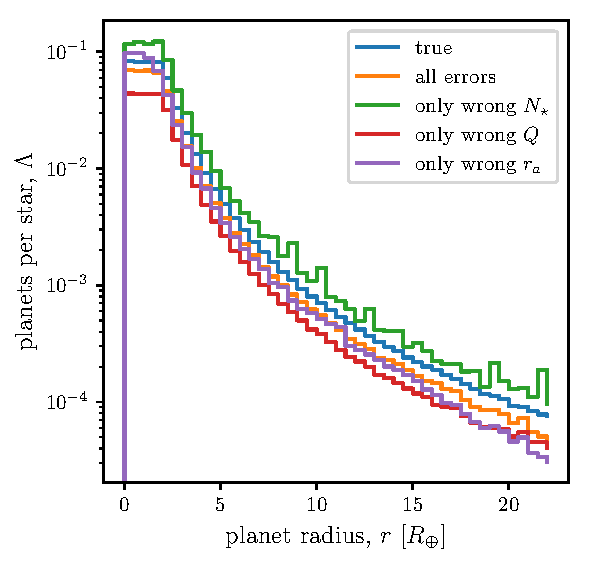
\includegraphics[width=.6\textwidth]{figures/errcases_rate_density_vs_radius_logs_model_3.pdf}
    \caption{
        Inferred planet occurrence rates as a function of planet radius in 
        Model 
        \#3.
        This model has fixed primaries and single stars, but varying 
        secondaries.
        The true planet radius distribution is a power law with exponent 
        $-2.92$ 
        above $2R_\oplus$, below which it is uniform (e.g., Howard et al., 
        2012).
    }
    \label{fig:errcases_model_3_log}
\end{figure}

\paragraph{Hot Jupiter Occurrence Rates}
Taking Fig.~\ref{fig:errcases_model_3_log} and counting the number of planets 
per star with $r>8r_\oplus$, we can compare the true and inferred hot Jupiter 
occurrence rates.
Under the above assumptions, the true rate is 9.1 hot Jupiters 
per thousand stars.
The inferred rate is 6.9 per thousand stars.
This means that the inferred rate underestimates the true rate by a 
multiplicative factor of $\sim\!1.3$.

However, this result only applies under the assumption that $Z_0 = 
Z_1 = Z_2$.
If hot Jupiters are less common around lower mass stars, it would be more 
sensible to consider $Z_2<Z_0$, while letting single stars and 
primaries host planets at the same rate.
Therefore in Fig.~\ref{fig:HJ_correction_inputrate_vs_HJratevalues} we let 
$Z_2$ vary, and show the resulting inferred and true hot Jupiter 
($r>8r_\oplus$) rates.
The result is that the inferred rate is nearly independent of 
$Z_2$~--~this is because most ($<1/10$) secondaries are not searchable, 
and so their completeness fraction is much smaller than that of primaries or 
single stars.
This means far fewer detected hot Jupiters orbit secondaries, and so they 
hardly affect the inferred rate.
While the ``true rate'' across the entire population is linearly dependent on 
$Z_2$, the rate around 
singles and primaries (green line) is independent of that around secondaries.
Assuming that RV surveys are measuring the true rate around single stars (or 
primaries), this suggests that binarity might contributes to the 
HJ rate discrepancy at the $\sim 0.2\%$ level, independent of the HJ rate 
around secondaries.


\begin{figure}[!tb]
    \centering
    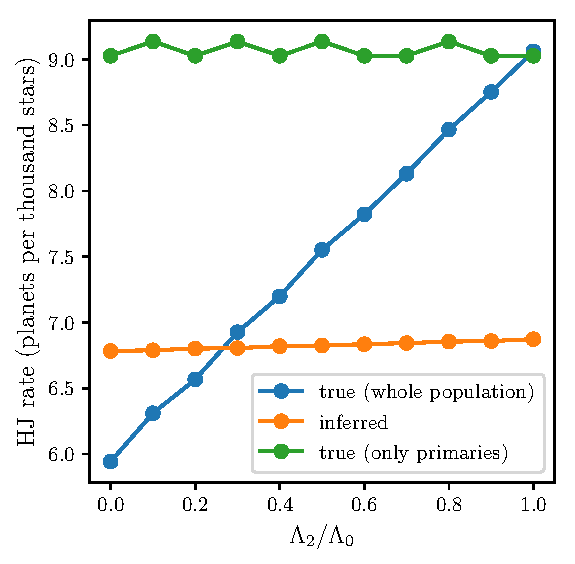
\includegraphics[width=.6\textwidth]{figures/HJ_correction_inputrate_vs_HJratevalues.pdf}
    \caption{
        $X_i$ is the occurrence rate integrated over all possible phase 
        space for the $i^{\rm th}$ system type. $Z_2/Z_0=1$ 
        corresponds to an equal number of planets per secondary as per single 
        star;
        $Z_2/Z_0=0$ corresponds to secondaries not having any 
        planets.
        In our Model \#3, though the true HJ occurrence rate 
        is highly dependent on $Z_2$, 
        the inferred rate hardly depends on whether secondaries have HJs.
        This means that the ``correction factor'' between the inferred rate 
        and the true rate around single stars is underestimated by a 
        multiplicative 
        factor of $\approx1.3$, independent of the HJ rate around secondaries.
        The ``HJ rate'' is the summed rate from     
        Fig.~\ref{fig:errcases_model_3_log} above $8r_\oplus$.
    }
    \label{fig:HJ_correction_inputrate_vs_HJratevalues}
\end{figure}


\paragraph{The Rate of Earth Analogs}
The rate (density) of Earth-like planets orbiting Sun-like stars has 
been independently measured by Youdin, Petigura, Dong \& Zhu, 
Foreman-Mackey et al., and Burke et al., (2011, 2013, 2013, 2014, and 2015 
respectively).
These efforts have found that the one-year terrestrial planet occurrence rate 
varies between $\approx 0.03$ and $\approx 1$ per Sun-like star, depending on 
assumptions that are made when retrieving the rate (Burke et al. 2015's 
Fig.~17).

Our model does not explicitly include the rate density's period-dependence, 
because stellar binarity does not appreciably bias the period-dependence of 
occurrence rates measured by transit surveys\footnote{
    Note that stellar binarity does bias the {\it intrinsic} planet 
    occurrence as a function of planetary and binary periods. This is expected 
    from dynamical stability limits in $\geq$3 body systems, and has been 
    observationally confirmed (theory by Holman \& Wiegert 1999, and others 
    including Gongjie; confirmation from Wang et al 2014a, 2014b, Kraus et al 
    2014). 
    However our statement is that inferred rates as a function of planet     
    period should be negligibly affected by this, given the geometric bias 
    against long-period transit detections, and the fact that the period 
    distribution of solar-type binaries peaks at $\approx 100\,{\rm years}$ 
    (Raghavan et al 2010, Fig.~13).
}.
Instead, it allows us to evaluate the difference in the apparent and true rate 
as a function of radius 
(Fig.~\ref{fig:errcases_model_3_log}).
At Earth's radius, the result is that the inferred rate is $0.84\times$ the 
true rate around single stars, assuming that the $Z_i$'s are equal.
Similar to the above case of the hot Jupiters, if we vary the true $Z_2$ 
while keeping $Z_0 = Z_1$, the ratio of the inferred to true rate 
around single stars hardly 
changes by only a few percent (shown in 
Fig.~\ref{fig:earth_inputrate_vs_etaearthratevalues}).
The ratio of the inferred to the true rate, $(\Lambda_{\rm 
inferred}/\Lambda)_{r=r_\oplus}$ varies substantially, but by at most $50\%$ 
in the (unrealistic) limiting case that secondaries do not host planets.


\begin{figure}[!tb]
    \centering
    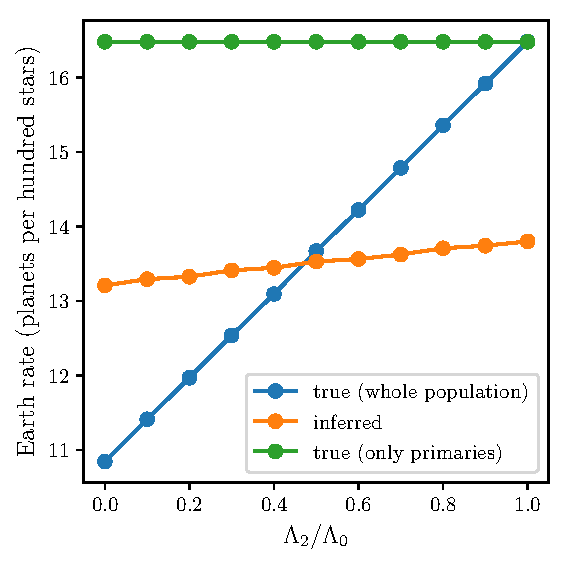
\includegraphics[width=.6\textwidth]{figures/earth_inputrate_vs_etaearthratevalues.pdf}
    \caption{
        Same as Fig.~\ref{fig:HJ_correction_inputrate_vs_HJratevalues}, but 
        for Earth-sized planets.
        The absolute values given on the $y$-axis found by summing the rate 
        from Fig.~\ref{fig:errcases_model_3_log} for planetary radii from 
        $0.5$ to $1.5r_\oplus$ (this is a toy model, and they do not reflect 
        an actual determination of $\eta_\oplus$).
        The relative values show that the inferred rate for Earths is roughly 
        independent of the occurrence rate (integrated over all radii) around 
        secondaries.
        However, it is systematically lower than the true rate around single 
        and primary stars, by $\approx 20\%$.
    }
    \label{fig:earth_inputrate_vs_etaearthratevalues}
\end{figure}
\section{Discussion}
\label{sec:discussion}

\paragraph{Does a detected planet orbit the primary or secondary?}
Ciardi et al. (2015) studied the effects of stellar multiplicity on the 
planet radii derived from transit surveys.
They modeled the problem for {\it Kepler}\ objects of interest by matching a 
population of binary and tertiary companions to KOI stars, 
under the assumption that the KIC-listed stars were the primaries.
They then computed planet radius correction factors assuming that {\it 
Kepler}-detected planets orbited the primary or companion stars
with equal probability (their Sec. 5).
Under these assumptions, they found that any given planet's radius is on 
average underestimated by a multiplicative factor of 1.5.

Our models show that assuming a detected planet has equal probability of 
orbiting the primary or secondary leads to an overstatement of
binarity's population-level effects.
A planet orbiting the secondary does lead to extreme corrections, but these 
cases are rare outliers, because the searchable volume for secondaries is so 
much smaller than that for primaries.
Phrased in terms of the completeness, in our Model \#3 only $\sim 6\%$ of 
selected secondaries are searchable, compared to $\sim 60\%$ of selected 
primaries.
This means that when high-resolution imaging discovers a binary companion in 
system that hosts a detected transiting planet, the planet is much
more likely to orbit the primary.
This statement is independent of the fact that planets are often confirmed to 
orbit the primary by inferring the stellar density from the transit duration.


\paragraph{On the utility for future occurrence rate measurements}
Though they will be difficult to distinguish from false positives, {\it TESS}\ 
is expected to discover over $10^4$ giant planets (Sullivan et al. 2015).
One possible use of this overwhelmingly large sample will to measure an
occurrence rate of short-period giant planets.
Our work indicates that if this measurement is to be more precise than $\sim 
30\%$, binarity cannot be neglected.


\paragraph{What about {\it Kepler}?}
Barclay \& Collaborator (in preparation) have performed the exercise 
of taking stars selected by the {\it Kepler}\ team, pairing them with a 
population of secondaries, injecting a realistic distribution of planet radii, 
and then comparing the inferred occurrence rates with the true ones.
In their model, they find that binarity leads to an inferred rate of 
Earth-sized planets $\approx 10\%$ less than the true rate.
In our Model \#3, if all $\Lambda_i$'s are equal (a plausible assumption in 
the lack of evidence to the contrary), the underestimate is by 16\%.

\section{Conclusion}
\label{sec:conclusion}

This study presented three simple models for the effects of binarity on 
occurrence rates measured by transit surveys.
The most realistic of these models (Model \#3) suggests that binarity does 
lead to underestimates in transit survey occurrence rates, but with less than 
$30\%$ relative error.
The model further suggests that hot Jupiter rates measured by transit surveys 
are biased to infer $\approx 1.3\times$ fewer hot Jupiters per star than 
surveys that only measure occurrence rates about single stars ({\it 
i.e..,} radial velocity surveys).
It also indicates that binarity's effects on the measured 
occurrence rates of Earth-sized planets are far smaller than current 
systematic uncertainties.
Though our models are simplistic, their agreement with Barclay \& 
Collaborator's recent detailed simulations indicate that they may capture the 
essential ingredients.


%\acknowledgements
%It was a pleasure to share discussions with Kento Masuda, who pointed us in 
%this direction, and helped clarify that something like this was worth studying.

%% \begin{deluxetable}{} command tell LaTeX how many columns
%% there are and how to align them.
\begin{deluxetable}{cccc}
    
%% Keep a portrait orientation

%% Over-ride the default font size
%% Use Default (12pt)

%% Use \tablewidth{?pt} to over-ride the default table width.
%% If you are unhappy with the default look at the end of the
%% *.log file to see what the default was set at before adjusting
%% this value.

%% This is the title of the table.
\caption{Occurrence rates of hot Jupiters (HJs) about FGK dwarfs, as measured 
by radial velocity and transit surveys.}
\label{tab:hj_rates}

%% This command over-rides LaTeX's natural table count
%% and replaces it with this number.  LaTeX will increment 
%% all other tables after this table based on this number
\tablenum{1}

%% The \tablehead gives provides the column headers.  It
%% is currently set up so that the column labels are on the
%% top line and the units surrounded by ()s are in the 
%% bottom line.  You may add more header information by writing
%% another line between these lines. For each column that requries
%% extra information be sure to include a \colhead{text} command
%% and remember to end any extra lines with \\ and include the 
%% correct number of &s.
\tablehead{\colhead{Reference} & \colhead{HJs per thousand stars} & 
\colhead{HJ Definition} 
%& 
%\colhead{} \\ 
%    \colhead{} & \colhead{(planets per thousand stars)} & \colhead{} & 
%    \colhead{}
} 

%% All data must appear between the \startdata and \enddata commands
\startdata
Marcy+ 2005 & 12$\pm$1 & $a<0.1\,{\rm AU}; P\lesssim10\,{\rm day}$ \\
Cumming+ 2008 & 15$\pm$6 & -- \\
Mayor+ 2011 & 8.9$\pm$3.6 & -- \\
Wright+ 2012 & 12.0$\pm$3.8 & -- \\
Gould+ 2006 & $3.1^{+4.3}_{-1.8}$ & $P<5\,{\rm day}$ \\
Bayliss+ 2011 & $10^{+27}_{-8}$ & $P<10\,{\rm day}$ \\
Howard+ 2012 & 4$\pm$1 & $P<10\,{\rm day}; r_p=8-32r_\oplus$; solar 
subset\tablenotemark{a} \\
-- & 5$\pm$1 & solar subset extended to $Kp<16$ \\
-- & 7.6$\pm$1.3 & solar subset extended to $r_p>5.6r_\oplus$. \\
Moutou+ 2013 & 10$\pm$3 & {\it CoRoT} average; $P\lesssim 10\,{\rm day}$, 
$r_p>4r_\oplus$  \\
Petigura+ (in prep) & 5.7$\pm$1.3 &
    $r_p=8-24r_\oplus$; $1<P/{\rm day}<10$; CKS stars\tablenotemark{b} \\
Santerne+ (in prep) & 9.5$\pm$2.6 & {\it CoRoT} galactic center \\
-- & 11.2$\pm$3.1 & {\it CoRoT} anti-center \\
\enddata

%% Include any \tablenotetext{key}{text}, \tablerefs{ref list},
%% or \tablecomments{text} between the \enddata and 
%% \end{deluxetable} commands

%% General table comment marker
\tablecomments{
    The upper four results are from radial velocity surveys; the rest
    are from transit surveys. Many of these surveys selected different 
    stellar samples. ``--'' denotes ``same as above''.
}
\tablenotetext{a}{
    Howard+ 2012's ``solar subset'' was defined as {\it Kepler}-observed stars 
    with $4100\,{\rm K}<T_{\rm eff}<6100\,{\rm K}$, $Kp <15$, $4.0 < \log g < 
    4.9$. Their rate selected planets with measured signal to noise $>10$.
    }
\tablenotetext{b}{
    Petigura+ (in prep)'s CKS subset included $\ldots$
}   
\end{deluxetable}


\end{document}
